\clearpage
\section{Sacred Vessels, Communion Arrangement, and Holy Oils}
\PCDPlateHeader{Plate III --- Sacred Vessels and Vessels for Communion}{Not to common scale}
\ifdefined\TriptychPrintEdition
\begin{center}
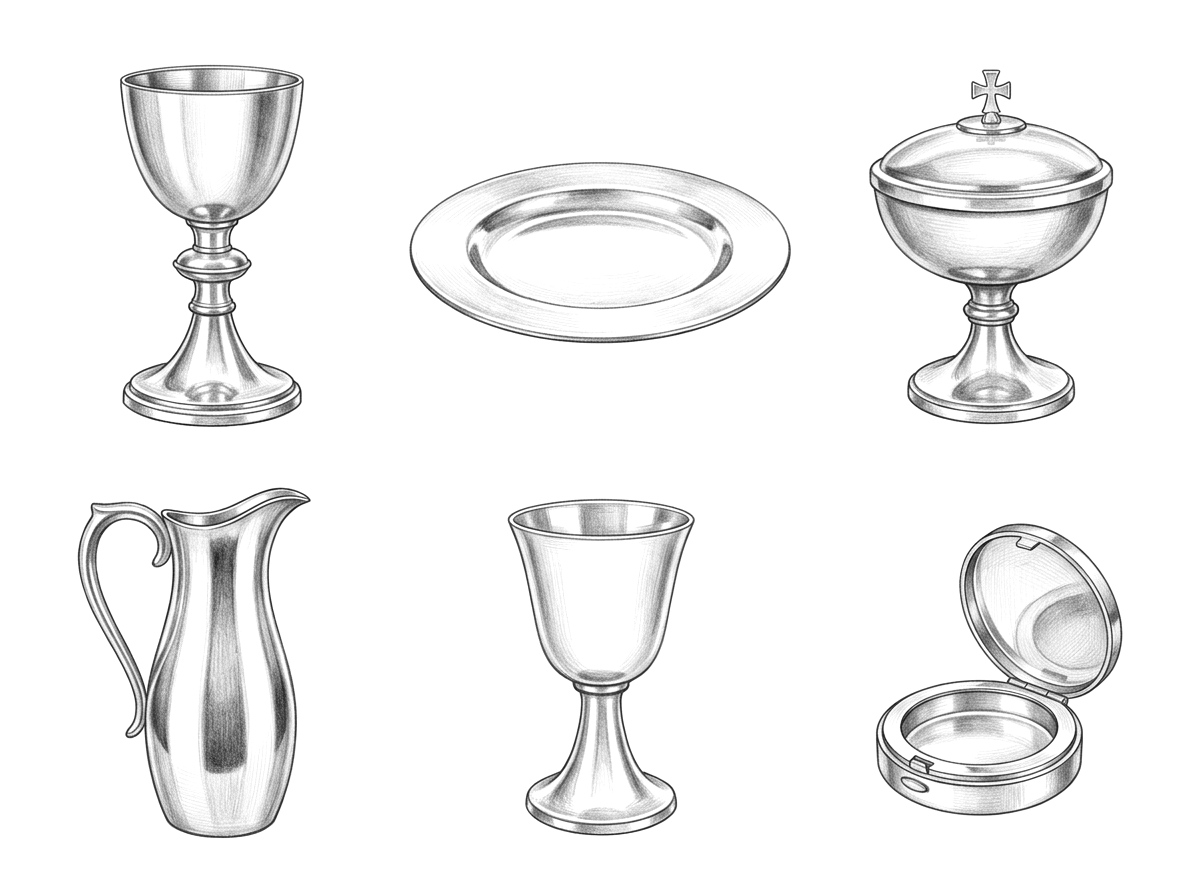
\includegraphics[width=0.92\linewidth,height=3.55in,keepaspectratio]{liturgy/roman-rite/postconciliar/2008-latin-2011-us-english/reference/roman-sanctuary-dictionary/shared/artwork/graphite/pc-art-03-sacred-vessels.png}
\end{center}
\PCDPositionKey{Top row, left to right: Chalice, wide shallow Paten, lidded footed Ciborium with cross finial. Bottom row, left to right: pitcher-style wine Flagon (pre-consecration transport only), footed Communion Cup (chalice), hinged pocket Pyx shown open.}
\else
\textbf{Visual Plate Summary (Plate III --- Sacred Vessels and Vessels for Communion, Not to common scale):} Six-vessel monochrome graphite comparison rendered with metallic reflections on white ground: top row left to right, a classical footed chalice with node, a broad shallow paten dish, and a lidded footed ciborium topped by a small cross; bottom row left to right, a tall slender pitcher-style wine flagon for bringing unconsecrated wine, a simpler footed Communion cup for distributing the Precious Blood, and a small hinged circular pocket pyx open to show its smooth gilded cavity.

\textbf{Reading order and object placement:} Top row, left to right: Chalice, wide shallow Paten, lidded footed Ciborium with cross finial. Bottom row, left to right: pitcher-style wine Flagon (pre-consecration transport only), footed Communion Cup (chalice), hinged pocket Pyx shown open.
\fi

\label{pc-obj-chalice}
\PCDEntryHead{Chalice}{Calix}{required}{N08}
\PCDField{Also called}{Principal Chalice; Eucharistic Chalice; \textit{Calix principalis}}
Verify that the chalice has been blessed (GIRM 333), that its interior gilding is intact and clean, and that no porous or breakable vessel (glass, ceramic, or clay) is ever substituted (GIRM 328, 330; RS 117). Prepare it on the credence table with a clean folded purificator, paten, optional pall, and---where customary---a white or seasonal chalice veil (GIRM 118c). After Mass, leave any unpurified chalice suitably covered on a corporal strictly for the priest, deacon, or instituted acolyte to purify before ordinary washing (GIRM 279; USCCB Norms 53).

\PCDField{Plate position and norm}{Top left (Plate III); center of the unfolded corporal (Plate X) (Universal Roman law)}
\PCDField{Placement and use}{Before Mass with a congregation, the chalice stands prepared on the credence table with the corporal, purificator, optional pall, and---as a praiseworthy practice commended in GIRM 118c---covered with a chalice veil of the color of the day or white (GIRM 118c). At the Preparation of the Gifts, the deacon, instituted acolyte, or server brings it to the altar, where the priest or deacon pours wine and a little water into it (GIRM 139, 142, 178). After the consecration, the priest elevates the chalice and the deacon elevates it during the final doxology (GIRM 150--151, 180). Following Communion, any remaining Precious Blood is consumed reverently at the altar and the chalice is purified strictly by the priest, deacon, or instituted acolyte---never poured into the sacrarium or ground (GIRM 279; RS 119; USCCB Norms 52--55). Every chalice is blessed before liturgical use according to the Roman Ritual, praiseworthily by the diocesan bishop or by a priest (GIRM 333; RS 118).}
\PCDField{United States norm}{While USCCB GIRM 329 permits solid, noble, non-breaking, non-absorbent materials such as hard woods for patens, ciboria, and pyxes, universal law requires the chalice bowl to be completely nonabsorbent (GIRM 330) and precious metal gilded inside if the metal rusts or is less precious than gold (GIRM 328); glass, earthenware, and clay chalices are strictly reprobated (Redemptionis Sacramentum 117).}
\PCDField{Prepared and handled by}{Prepares: Sacristan, Deacon, Instituted acolyte, Altar server. Ministers in use: Bishop, Priest, Deacon.}
\PCDSafety{Once consecrated, the chalice contains the Blood of Christ: servers and extraordinary ministers never purify it (strictly reserved to priest, deacon, or instituted acolyte), and remaining Precious Blood is never poured into the sacrarium or onto the ground (USCCB Norms 53--55).}
\PCDField{Distinguish from}{Communion Cup, Ciborium, Flagon}
\PCDEntryRule

\label{pc-obj-paten}
\PCDEntryHead{Paten}{Patena}{required}{N09}
\PCDField{Also called}{Eucharistic Paten; Large Paten; \textit{Patena maior}}
Confirm that the paten has been blessed (GIRM 333) and is made of precious metal (GIRM 328) or an approved solid non-breaking, non-absorbent material such as hardwood under USCCB GIRM 329---never earthenware, clay, or glass (RS 117). Size the paten generously when the parish uses a single large host broken for concelebrants and faithful (GIRM 331), and place the separate Communion-plate cleanly on the credence table whenever it is used (GIRM 118c; RS 93).

\PCDField{Plate position and norm}{Top center (Plate III); front center of the unfolded corporal (Plate X) (Universal Roman law)}
\PCDField{Placement and use}{Universal Roman law recommends a paten sufficiently wide to hold the Eucharistic bread not only for the priest and deacon, but also for the other ministers and the faithful, manifesting the unity of the one bread (GIRM 331). Before the Preparation of the Gifts, the paten rests either on the credence table or in the Procession of the Gifts; during the Eucharistic Prayer it rests on the unfolded corporal (GIRM 118c, 139, 306). After Communion, any particles are carefully gathered and the paten is purified strictly by the priest, deacon, or instituted acolyte (GIRM 278--279; RS 119). Distinguish the Eucharistic paten holding the host from the separate Communion-plate (patina pro Communione fidelium), retained by GIRM 118c and Redemptionis Sacramentum 93 to be held beneath communicants' chins so no fragment falls.}
\PCDField{United States norm}{Under the United States adaptation to GIRM 329, patens (along with ciboria and pyxes) may be crafted either from precious metal (GIRM 328) or from other solid, noble materials such as ebony or hard woods that do not break easily, deteriorate, or absorb liquids.}
\PCDField{Prepared and handled by}{Prepares: Sacristan, Deacon, Instituted acolyte, Altar server. Ministers in use: Bishop, Priest, Deacon.}
\PCDSafety{If holding a Communion-plate during Holy Communion, keep it completely level beneath each communicant's chin without tipping it, and hand it back to the priest, deacon, or instituted acolyte at the altar or credence table so any particles are purified properly.}
\PCDField{Distinguish from}{Ciborium, Pyx}
\PCDEntryRule

\label{pc-obj-ciborium}
\PCDEntryHead{Ciborium}{Pyxis}{provided}{N10}
\PCDField{Also called}{Host Vessel; Covered Ciborium; \textit{Ciborium}; \textit{Vas}}
Ensure every ciborium is blessed (GIRM 333), clean, dry, and fitted with a tight cover if used for reservation in the tabernacle (CIC can. 939). Check that porous earthenware, clay, and glass vessels are excluded (RS 117), and rotate reserved hosts regularly so consecrated hosts remain fresh. Leave used ciboria covered on a corporal after Mass for purification exclusively by the priest, deacon, or instituted acolyte (GIRM 279; USCCB Norms 53).

\PCDField{Plate position and norm}{Top right (Plate III); draped in a white veil at rear right of the corporal (Plate X) (Universal Roman law)}
\PCDField{Placement and use}{The Latin third typical edition of the General Instruction uses pyxis / pyxides (GIRM 118c, 306, 329; CIC can. 939) where the official English text renders ``ciborium'' and ``ciboria.'' Unconsecrated ciboria holding hosts for the congregation are prepared on the credence table or carried in the Procession of the Gifts, and empty ciboria may be brought to the altar at the Fraction Rite if needed for distribution (GIRM 118c, 139; USCCB Norms 37). Any ciborium used for tabernacle reservation requires a fitted cover, and reserved hosts must be renewed frequently (CIC can. 939). A white silk veil (conopaeum) over a reserved ciborium remains a reverent custom though not universally mandated by GIRM. Every ciborium is blessed before use (GIRM 333) and purified after Communion strictly by the priest, deacon, or instituted acolyte (GIRM 279; RS 119; USCCB Norms 53).}
\PCDField{United States norm}{While universal law prescribes precious metal gilded inside where less precious than gold (GIRM 328), the United States adaptation at GIRM 329 permits ciboria to be crafted from other solid, noble, non-breaking, non-absorbent materials such as ebony or hard woods; fragile ceramic, clay, and glass remain strictly prohibited (Redemptionis Sacramentum 117).}
\PCDField{Prepared and handled by}{Prepares: Sacristan, Deacon, Instituted acolyte, Altar server. Ministers in use: Bishop, Priest, Deacon, Instituted acolyte, Extraordinary minister of Holy Communion.}
\PCDSafety{Never open, lift, or carry a ciborium containing the Blessed Sacrament unless ordained, instituted as an acolyte, or formally deputed as an extraordinary minister of Holy Communion for distribution; never wash an unpurified ciborium.}
\PCDField{Distinguish from}{Chalice, Paten, Pyx}
\PCDEntryRule

\label{pc-obj-pyx}
\PCDEntryHead{Pyx}{Pyxis parva}{provided}{N11}
\PCDField{Also called}{Sick-Call Pyx; Pocket Pyx; \textit{Theca}; \textit{Pyxis}}
Keep parish pyxes clean, dry, securely latching, and blessed (GIRM 333), stored together with small clean sick-call corporals and carrying pouches. Verify that pyxes brought forward for homebound ministry belong to authorized ministers and remind ministers to return empty pyxes properly purified rather than leaving fragments inside.

\PCDField{Plate position and norm}{Bottom right, shown hinged open to display the recessed interior (Plate III) (Universal Roman law)}
\PCDField{Placement and use}{Kept clean and empty in the sacristy or with the sick-call kit until needed, a pyx is blessed before liturgical use (GIRM 333; RS 118). Consecrated hosts are placed in it by a bishop, priest, deacon, instituted acolyte, or formally deputed extraordinary minister of Holy Communion strictly for an authorized pastoral visit to the sick---never placed casually in an unauthorized private container (CIC can. 939; Holy Communion and Worship of the Eucharist Outside Mass; RS 133). After Communion of the sick, the pyx is purified reverently with water so no particle of the Host remains.}
\PCDField{United States norm}{United States GIRM 329 explicitly enumerates pyxes among the sacred vessels governed by the noble, solid, non-breaking, non-absorbent material standard.}
\PCDField{Prepared and handled by}{Prepares: Sacristan, Priest, Deacon. Ministers in use: Bishop, Priest, Deacon, Instituted acolyte, Extraordinary minister of Holy Communion.}
\PCDSafety{A closed pyx may contain the Body of Christ. Never open an unattended pyx or place it in ordinary storage; report any closed pyx found in the sanctuary or sacristy immediately to the priest or deacon.}
\PCDField{Distinguish from}{Ciborium, Paten}
\PCDEntryRule

\label{pc-obj-communion-cup}
\PCDEntryHead{Communion Cup}{Calix}{territorial adaptation}{N12}
\PCDField{Also called}{Communion Chalice; Additional Chalice; \textit{Calix ad Communionem sub utraque specie}}
Set out the exact number of blessed Communion chalices needed for the congregation, paired one-for-one with clean folded purificators (GIRM 286; USCCB Norms 35). Inspect interior gilding and verify no glass, ceramic, or clay cups are ever used (GIRM 330; RS 117). Estimate wine quantities carefully before Mass so all wine is poured into chalices before the Eucharistic Prayer without excess remaining Precious Blood afterward (RS 106). After Mass, leave unpurified cups covered on a corporal exclusively for the priest, deacon, or instituted acolyte (GIRM 279; USCCB Norms 53).

\PCDField{Plate position and norm}{Bottom center (Plate III); flanking the principal chalice beside folded purificators (Plate X) (USCCB territorial adaptation)}
\PCDField{Placement and use}{Every Communion cup is a true liturgical chalice and must be blessed before use and crafted with a nonabsorbent bowl---precious metal gilded inside if less precious than gold, never glass, earthenware, clay, or common domestic tableware (GIRM 328, 330, 333; RS 117--118; USCCB Norms 35). Wine is poured into all Communion chalices at the Preparation of the Gifts before the Eucharistic Prayer begins; pouring the Precious Blood from a flagon or from one chalice into another after consecration is strictly forbidden (RS 106; USCCB Norms 35--38). Each chalice is accompanied by a clean purificator to wipe the rim after each communicant (GIRM 286). After Communion, remaining Precious Blood is immediately consumed at the altar by the bishop, priest, deacon, or instituted acolyte---or by an extraordinary minister from his or her own chalice only with the diocesan bishop's permission---and all cups are purified strictly by the priest, deacon, or instituted acolyte (GIRM 279; RS 119; USCCB Norms 52--53).}
\PCDField{United States norm}{Under GIRM 283 and the USCCB Norms for the Distribution and Reception of Holy Communion under Both Kinds in the Dioceses of the United States of America (2002; revised 2011), Communion from the chalice is broadly extended across United States dioceses. Liturgical law treats every Communion cup as a chalice governed by full sacred-vessel standards (GIRM 328, 330; RS 117).}
\PCDField{Prepared and handled by}{Prepares: Sacristan, Deacon, Instituted acolyte, Altar server. Ministers in use: Bishop, Priest, Deacon, Instituted acolyte, Extraordinary minister of Holy Communion.}
\PCDSafety{Strict liturgical law: wine must be poured into Communion cups before consecration---never pour the consecrated Precious Blood from a flagon or between chalices (RS 106). Following the October 2006 non-renewal of the temporary U.S. indult, extraordinary ministers and altar servers never purify Communion cups; purification is reserved strictly to priest, deacon, or instituted acolyte (USCCB Norms 53).}
\PCDField{Distinguish from}{Chalice, Flagon, Ciborium}
\PCDEntryRule

\label{pc-obj-cruets}
\PCDEntryHead{Cruets}{Urceoli}{required}{N13}
\PCDField{Also called}{Wine and Water Cruets; \textit{Ampullae}; \textit{Urceoli cum vino et aqua}}
Fill the wine cruet with valid natural grape wine (pure, unspoiled, free of foreign substances, CIC can. 924 §3) and the water cruet with fresh clean water, setting both on a small tray on the credence table (GIRM 118c). Keep stoppers clean to guard against dust or insects, and wash glass cruets thoroughly after Mass so no dried wine residue accumulates.

\PCDField{Plate position and norm}{See Plate VI, top left (paired with stoppers on an oval metal tray); Plate I, atop the credence table (Universal Roman law)}
\PCDField{Placement and use}{Before Mass, the cruets of wine and water are prepared on the credence table (unless the wine is brought forward in the Procession of the Gifts, in which case the water cruet still remains ready on the credence table: GIRM 118c, 140). At the Preparation of the Gifts, the server or instituted acolyte brings the cruets to the deacon or priest at the altar, who pours wine and a few drops of water into the chalice (GIRM 142, 178, 190). After Communion, the server brings the water cruet again so the priest, deacon, or instituted acolyte may purify the paten, chalice, and ciboria (GIRM 163, 279). Because cruets hold unconsecrated elements and are not sacred vessels, clear glass is customary and helpful so ministers tell wine from water at a glance.}
\PCDField{Prepared and handled by}{Prepares: Sacristan, Altar server. Ministers in use: Priest, Deacon, Instituted acolyte, Altar server.}
\PCDSafety{Remove glass stoppers safely on the credence table before approaching the altar so stoppers are not dropped on stone steps; never leave cruets sitting on the altar table during the Eucharistic Prayer (GIRM 306).}
\PCDField{Distinguish from}{Flagon, Lavabo Towel}
\PCDEntryRule

\label{pc-obj-flagon}
\PCDEntryHead{Flagon}{Lagoena}{permitted}{N14}
\PCDField{Also called}{Wine Pitcher; Offertory Carafe; \textit{Lagena}; \textit{Ampulla maior}}
Fill the flagon with the measured quantity of valid grape wine required for the Communion chalices and place it on the gifts table in the nave before Mass. Never substitute a flagon for blessed Communion chalices on the altar: all wine to be consecrated must be poured into nonabsorbent blessed chalices before the Eucharistic Prayer begins (GIRM 306, 330; RS 106; USCCB Norms 35--38).

\PCDField{Plate position and norm}{Bottom left, tall slender pitcher with curved handle and pouring lip (Plate III) (Diocesan or local selection)}
\PCDField{Placement and use}{When a large assembly celebrates Communion under both kinds, representatives of the faithful may carry unconsecrated wine forward in a dignified flagon during the Procession of the Gifts (GIRM 73, 140). At the Preparation of the Gifts, the priest or deacon pours all wine intended for consecration from the flagon into the principal chalice and supplementary Communion chalices, and the empty flagon is removed immediately to the credence table before the Eucharistic Prayer starts (GIRM 306). A flagon is never a sacred vessel for consecration and never holds the Precious Blood: Redemptionis Sacramentum 106 forbids both containing the Blood of Christ in flagons or bowls and pouring the consecrated Precious Blood from one vessel into another.}
\PCDField{United States norm}{In United States parishes celebrating Communion under both kinds, a flagon is permitted strictly as a pre-consecration transport vessel in the Procession of the Gifts; Redemptionis Sacramentum 106 and the 2011 USCCB Norms strictly prohibit consecrating wine in a flagon or pouring the Precious Blood from a flagon into Communion cups after consecration.}
\PCDField{Prepared and handled by}{Prepares: Sacristan, Altar server. Ministers in use: Faithful, Priest, Deacon, Instituted acolyte, Altar server.}
\PCDSafety{Strict liturgical boundary (Redemptionis Sacramentum 106): never leave a flagon containing wine on the altar during the Eucharistic Prayer, never treat a flagon as a chalice, and never allow the consecrated Precious Blood to be poured from a flagon into Communion cups.}
\PCDField{Distinguish from}{Chalice, Communion Cup, Cruets}
\PCDEntryRule

\clearpage
\PCDPlateHeader{Plate X --- Communion Under Both Kinds and Sacramental Vessels}{Not to common scale}
\ifdefined\TriptychPrintEdition
\begin{center}
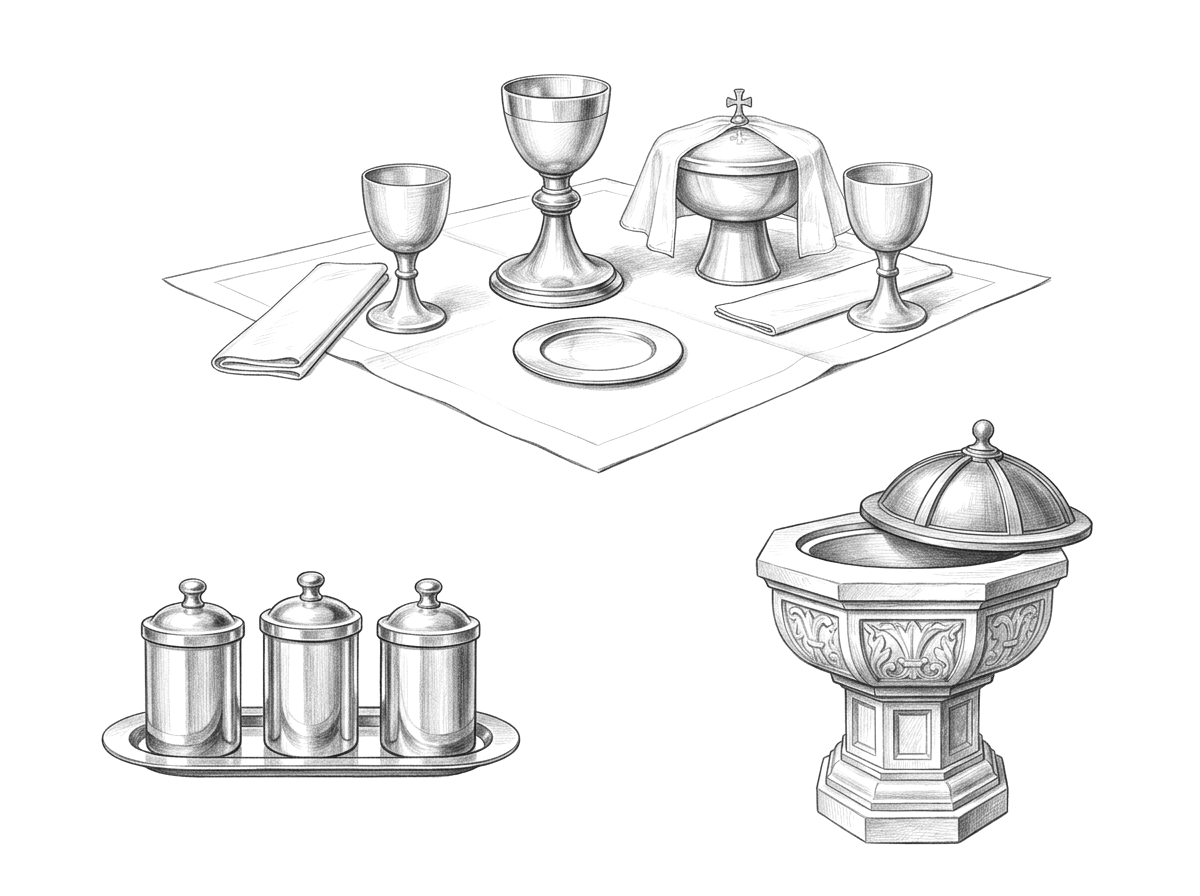
\includegraphics[width=0.92\linewidth,height=3.55in,keepaspectratio]{liturgy/roman-rite/postconciliar/2008-latin-2011-us-english/reference/roman-sanctuary-dictionary/shared/artwork/graphite/pc-art-10-communion-triduum-vessels.png}
\end{center}
\PCDPositionKey{Top: Communion under both kinds arrangement on an unfolded Corporal (principal Chalice, Paten, veiled covered Ciborium, and two footed Communion Cups each with a folded Purificator); bottom left: three cylindrical lidded metal Holy Oils Stocks on a tray (Sacred Chrism, Oil of Catechumens, Oil of the Sick); bottom right: carved octagonal stone Baptismal Font with removable domed cover ajar.}
\else
\textbf{Visual Plate Summary (Plate X --- Communion Under Both Kinds and Sacramental Vessels, Not to common scale):} Three-group monochrome graphite sacramental plate: top, an unfolded square corporal holding a central principal chalice, shallow paten, closed ciborium draped in a white veil, and two footed Communion cups each beside a folded purificator; bottom left, three matching cylindrical lidded metal holy-oil vessels resting on an oval metal tray without baked inscriptions; bottom right, an octagonal carved stone baptismal font on a pedestal with its domed cover resting slightly open to reveal the water basin rim.

\textbf{Reading order and object placement:} Top: Communion under both kinds arrangement on an unfolded Corporal (principal Chalice, Paten, veiled covered Ciborium, and two footed Communion Cups each with a folded Purificator); bottom left: three cylindrical lidded metal Holy Oils Stocks on a tray (Sacred Chrism, Oil of Catechumens, Oil of the Sick); bottom right: carved octagonal stone Baptismal Font with removable domed cover ajar.
\fi

\label{pc-obj-holy-oils-stocks}
\PCDEntryHead{Holy Oils and Oil Stocks}{Olea sancta et vasa oleorum}{required}{N40}
\PCDField{Also called}{Sacred Chrism (SC), Oil of Catechumens (OC), and Oil of the Sick (OI); oil stocks; chrismatory; oil urns; ambry (oil cabinet); \textit{Sanctum Chrisma}; \textit{Oleum catechumenorum}; \textit{Oleum infirmorum}; \textit{ampullae oleorum}; \textit{thecae}; \textit{armarium oleorum}}
Before the Chrism Mass, clean and thoroughly dry the parish urns and portable stocks, check that engraved abbreviations (SC/CHR for Sacred Chrism, OC---or older Latin OS, Oleum Sanctum, never to be confused with English ``Oil of the Sick''---for Oil of Catechumens, and OI/INF for Oil of the Sick) match cleanly on both body and lid, and replace oil-soaked cotton in pocket stocks with fresh absorbent cotton. After the fresh oils arrive, coordinate with the pastor to dispose of the previous year's oils reverently by burning or via the sacrarium or clean earth per diocesan direction---never down ordinary drains---and keep the ambry clean and locked (CIC can. 847, par. 2). Before Baptisms or Confirmations, set out the required stock alongside cotton, lemon, warm water, and a hand towel.

\PCDField{Plate position and norm}{Bottom left, three matching cylindrical lidded metal oil stocks on an oval tray (Plate X) (Universal Roman law)}
\PCDField{Placement and use}{At the annual Chrism Mass (Missa Chrismatis), celebrated on Holy Thursday morning or an earlier day in Holy Week close to Easter, the diocesan bishop blesses the Oil of the Sick and the Oil of Catechumens and mixes balsam or fragrance into oil to consecrate Sacred Chrism (Ordo benedicendi oleum 1970; Caeremoniale Episcoporum 1984 no. 274). Parishes receive fresh oils each year and reserve them under lock in a clean, dignified ambry in the sanctuary, baptistery, or sacristy (CIC can. 847, par. 2). Sacred Chrism anoints the newly baptized, the confirmed, newly ordained priests and bishops, and dedicated churches and altars; Oil of Catechumens is used in pre-baptismal anointing; and Oil of the Sick is administered in the Anointing of the Sick.}
\PCDField{United States norm}{Universal canon law (CIC can. 847) requires every parish to obtain newly consecrated and blessed oils each year from its diocesan bishop and safeguard them diligently. In the United States, parishes commonly receive the new oils during the Evening Mass of the Lord's Supper on Holy Thursday using the USCCB Order for the Reception of the Holy Oils, and many churches display the locked ambry visibly near the baptismal font or sanctuary.}
\PCDField{Prepared and handled by}{Prepares: Priest, Sacristan. Ministers in use: Bishop, Priest, Deacon.}
\PCDSafety{Never open an oil stock, attempt to anoint anyone, or interchange caps between SC, OC, and OI vessels. Hold closed oil urns upright with both hands during processions to prevent oil spills on sanctuary steps, and never discard previous year's oils in ordinary sinks, trash, or plumbing; old oils are burned reverently (commonly absorbed in cotton or consumed in the Easter fire) or poured into the sacrarium or clean earth according to diocesan direction.}
\PCDField{Distinguish from}{Pyx, Cruets}
\PCDEntryRule
